\section{Introduction}

\begin{definitionbox}
    \definition{Operations Research (OR)}, often shortened to the initialism \texttt{OR}, is the branch of mathematics in which \textbf{mathematical models} and \textbf{quantitative methods} (e.g. optimization, game theory, simulation) are \textbf{used to analyze complex decision-making problems} and \textbf{find (near-)optimal solutions}.
\end{definitionbox}

\highspace
The overall and primary \emph{goal} is to \emph{help make better decisions}.

\highspace
OR can be seen as an interdisciplinary field at the intersection of applied mathematics, computer science, economics, and industrial engineering.

\highspace
Operations research is often concerned with \textbf{determining the extreme values of some real-world objective}: the \emph{maximum} (of profit, performance, or yield) or \emph{minimum} (of loss, risk, or cost). Originating in military efforts before World War II, its techniques have grown to concern problems in a variety of industries.\cite{wikipediaOperationsResearch}

\highspace
Its origins date back to World War II: teams of scientists were asked to research the most efficient way to conduct operations (e.g., to optimize the allocation of scarce resources).

\highspace
In the decades after the war, the techniques became public and were applied more widely to problems in business, industry, and society.

\highspace
During the industrial boom, the substantial increase in the size of firms and organizations led to more complex decision problems.

\highspace
There are favorable circumstances: rapid progress in OR and in numerical analysis methods, and the advent and spread of computers (available computing power and widespread software).

\newpage

\subsection{Decision-making problems}

Decision-making problems are analyzed using mathematical models and quantitative methods.

\begin{definitionbox}
    \definition{Decision-making problems} are problems in which we must \textbf{choose} a (feasible) \textbf{solution among a large number of alternatives based on one or several criteria}.
\end{definitionbox}

\highspace
In other words, they are complex decision-making problems that are \textbf{addressed through a mathematical modeling approach} (mathematical models, algorithms, and computer implementations).

\highspace
Some practical \example{examples} include assignment problem, network design, shortest paths, personnel scheduling, service management, multicriteria problem, and maximum clique.

\longline

\subsubsection{Assignment problem}

A mathematical definition of an \definition{assignment problem} is as follows. Given $m$ jobs and $m$ machines, suppose that each job can be executed by any machine and that $t_{ij}$ is the execution time of job $J_{i}$ on machine $M_{j}$.

\begin{table}[!htp]
    \centering
    \begin{tabular}{@{} c | c c c @{}}
        & $M_{1}$ & $M_{2}$ & $M_{3}$ \\
        \cmidrule{1-4}
        $J_{1}$ & $2$ & $6$ & $3$ \\
        $J_{2}$ & $8$ & $4$ & $9$ \\
        $J_{3}$ & $5$ & $7$ & $8$
    \end{tabular}
    \caption{Example of an assignment problem table.}
\end{table}

\noindent
The \textbf{main goal} is to \textbf{decide which job to assign to each machine in order to minimize the total execution time}. Also, (constraints) each job must be assigned to exactly one machine, and each machine must be assigned to exactly one job.

\highspace
The \textbf{number} of feasible \textbf{solutions} is the permutations, then the \textbf{factorial of} $m$: $m!$.

\newpage

\subsubsection{Network design}

The \definition{network design problem} is characterized as \textbf{how to connect} $n$ \textbf{cities} (offices) \textbf{via a collection of possible links} so as (\emph{main goal}) \textbf{to minimize the total link cost}.

\highspace
Using mathematical terms, given a graph $G = \left(N,E\right)$ with a node $i \in N$ for each city and an edge $\left\{i,j\right\} \in E$ of cost $c_{ij}$, select a subset of edges of minimum total cost, guaranteeing that all pairs of nodes are connected.

\begin{figure}[!htp]
    \centering
    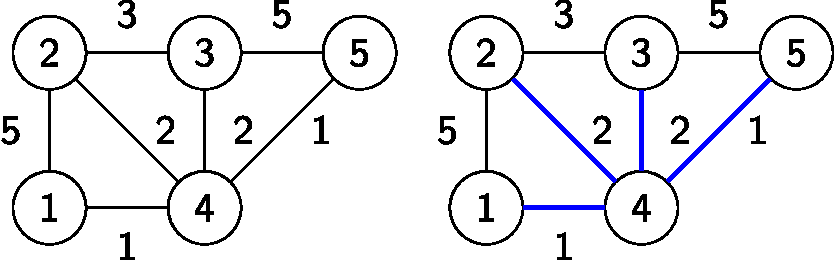
\includegraphics[width=.5\textwidth]{img/network-design-1.pdf}
    \caption{Examples of network design graphs.}
\end{figure}

\noindent
The \textbf{number} of alternative \textbf{solutions} is at most $2^{m}$, where $m = \left|E\right|$.

\longline

\subsubsection{Shortest path}

The \definition{shortest path problem} is similar to network design. Given a direct path that represents a road network with distances (traveling times) for each arc, determine the shortest (fastest) path between two points (nodes).

\begin{figure}[!htp]
    \centering
    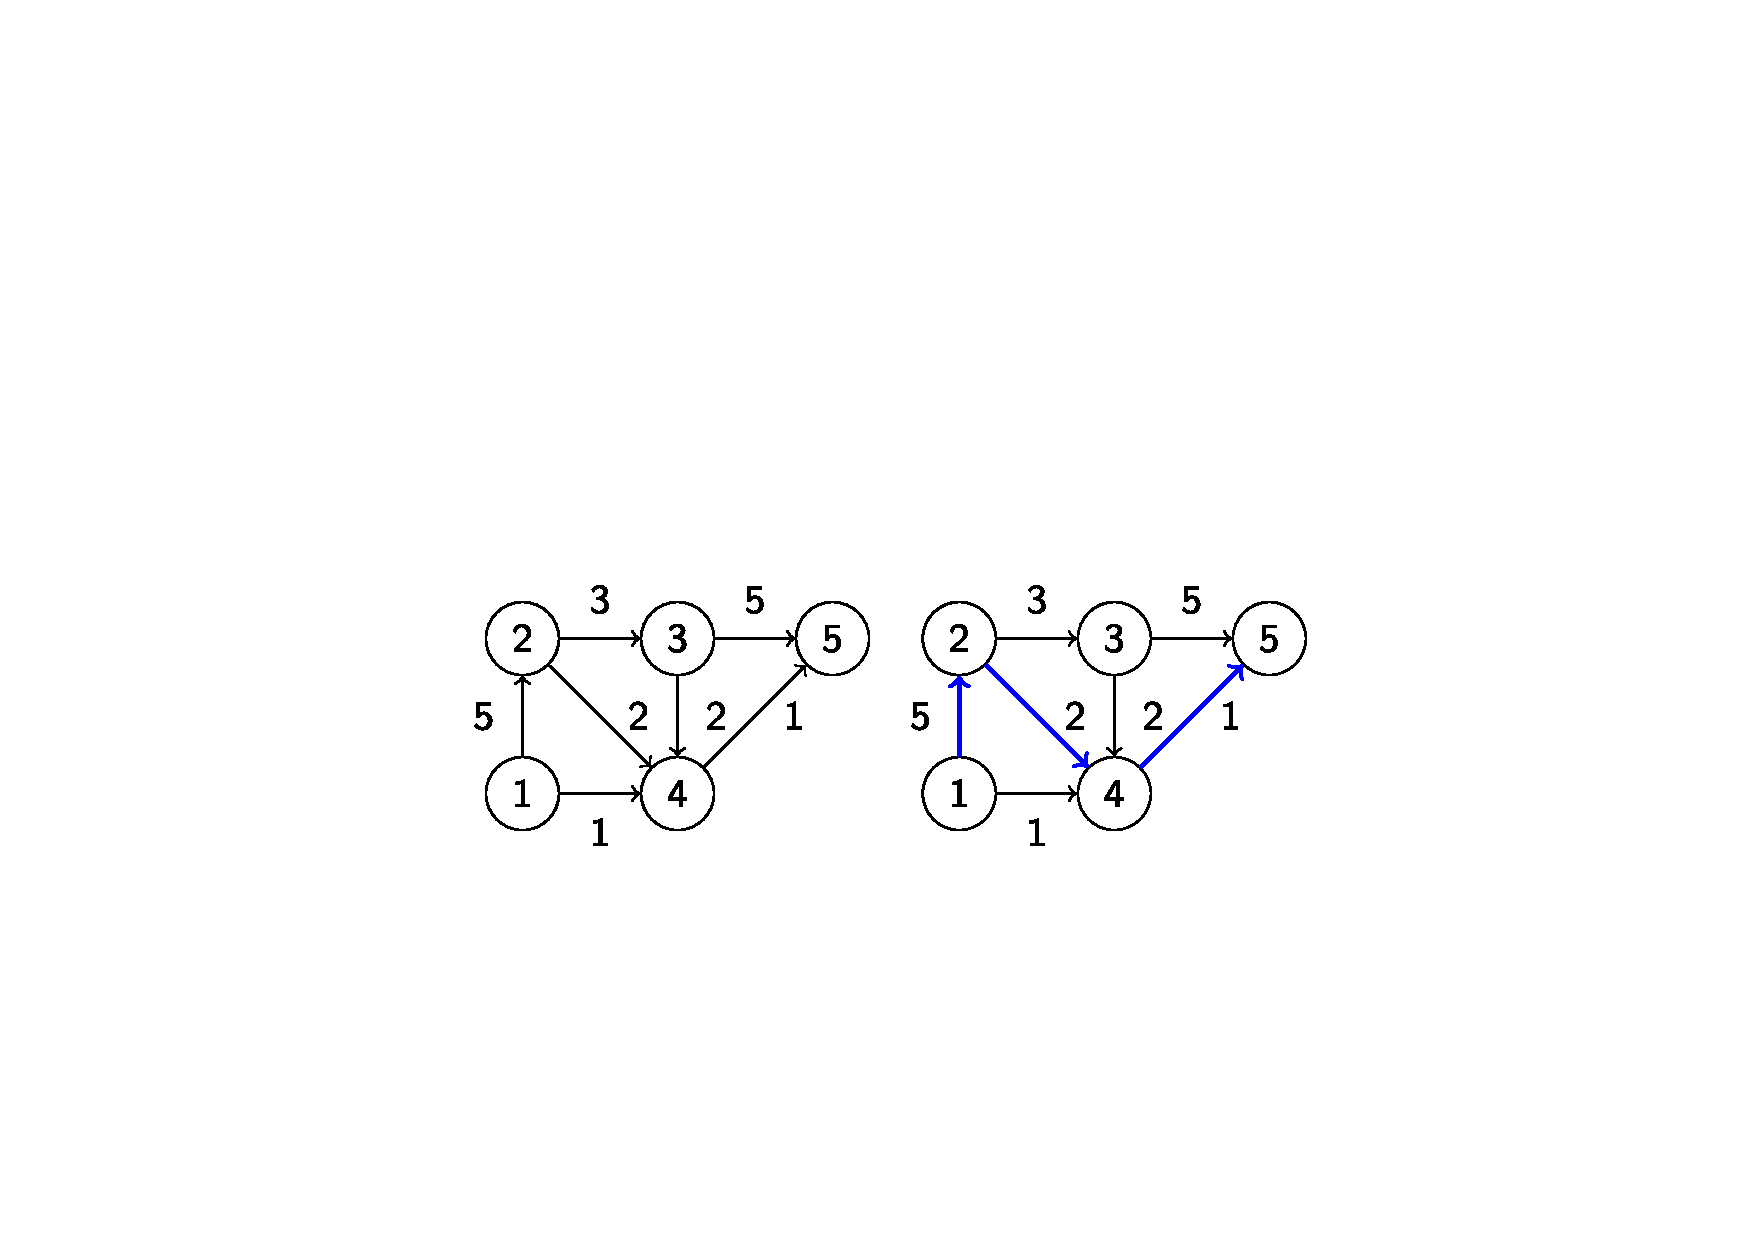
\includegraphics[width=.5\textwidth]{img/shortest-path-1.pdf}
    \caption{Examples of shortest path graphs.}
\end{figure}

\longline

\subsubsection{Other problems}

Other decision-making problems are:
\begin{itemize}
    \item \definition{Personnel scheduling problem}: determine the week schedule for the hospital personnel, so as to minimize the number of people involved (physicians, nurses, \dots) while meeting the daily requirements.
    
    \item \definition{Service management problem}: determine how many counters/desks to open at a given time of the day so that the average customer waiting time does not exceed a certain value (guarantee a given service quality).

    \item \definition{Multicriteria problem}: decide which laptop to buy considering the price, the weight and the performance.

    \item \definition{Maximum clique problem}: determine the complete subgraph of a graph, with maximum number of vertices.
\end{itemize}